\documentclass[10pt,fleqn]{article} % Default font size and left-justified equations
\usepackage[%
    pdftitle={Centrale Supelec 2018},
    pdfauthor={UPSTI}]{hyperref}

\input{style/new_style}
%%%%%%%%%%%%
% Définition des vecteurs 
%%%%%%%%%%%%

\newcommand{\vect}[1]{\overrightarrow{#1}}
\newcommand{\axe}[2]{\left(#1,\vect{#2}\right)}
\newcommand{\couple}[2]{\left(#1,\vect{#2}\right)}
\newcommand{\angl}[2]{\left(\vect{#1},\vect{#2}\right)}

\newcommand{\rep}[1]{\mathcal{R}_{#1}}
\newcommand{\bas}[1]{\mathcal{B}_{#1}}
\newcommand{\quadruplet}[4]{\left(#1;#2,#3,#4 \right)}
\newcommand{\repere}[4]{\left(#1;\vect{#2},\vect{#3},\vect{#4} \right)}
\newcommand{\base}[3]{\left(\vect{#1},\vect{#2},\vect{#3} \right)}


\newcommand{\vx}[1]{\vect{x_{#1}}}
\newcommand{\vy}[1]{\vect{y_{#1}}}
\newcommand{\vz}[1]{\vect{z_{#1}}}
\newcommand{\vi}[1]{\vect{i_{#1}}}
\newcommand{\vj}[1]{\vect{j_{#1}}}
\newcommand{\vk}[1]{\vect{k_{#1}}}
\newcommand{\vAB}{\vect{AB}}
\newcommand{\vBA}{\vect{BA}}
\newcommand{\vBC}{\vect{BC}}
\newcommand{\vCB}{\vect{CB}}
\newcommand{\vCA}{\vect{CA}}
\newcommand{\vAC}{\vect{AC}}


% d droit pour le calcul différentiel
\newcommand{\dd}{\text{d}}
\newcommand{\deriv}[2]{ \dfrac{ \dd }{\dd t} \left[  #1\right]_{#2}}
\newcommand{\dderiv}[2]{ \dfrac{ \dd^2 }{\dd t^2} \left[  #1\right]_{#2}}

% dérivée
\newcommand{\varphip}{\dot{\varphi}}
\newcommand{\thetap}{\dot{\theta}}
\newcommand{\lambdap}{\dot{\lambda}}
\newcommand{\varphipp}{\ddot{\varphi}}
\newcommand{\thetapp}{\ddot{\theta}}
\newcommand{\lambdapp}{\ddot{\lambda}}



\newcommand{\inertie}[2]{I_{#1}\left( #2\right)}
\newcommand{\matinertie}[7]{
\begin{pmatrix}
#1 & #6 & #5 \\
#6 & #2 & #4 \\
#5 & #4 & #3 \\
\end{pmatrix}_{#7}}
%%%%%%%%%%%%
% Définition des torseurs 
%%%%%%%%%%%%

\newcommand{\ec}[2]{%
\mathcal{E}_c\left(#1/#2\right)}

\newcommand{\pext}[3]{%
\mathcal{P}\left(#1\rightarrow#2/#3\right)}

\newcommand{\pint}[3]{%
\mathcal{P}\left(#1 \stackrel{\text{#3}}{\leftrightarrow} #2\right)}


 \newcommand{\torseur}[1]{%
\left\{{#1}\right\}
}

\newcommand{\torseurcin}[3]{%
\left\{\mathcal{#1} \left(#2/#3 \right) \right\}
}

\newcommand{\torseurci}[2]{%
%\left\{\sigma \left(#1/#2 \right) \right\}
\left\{\mathcal{C} \left(#1/#2 \right) \right\}
}
\newcommand{\torseurdyn}[2]{%
\left\{\mathcal{D} \left(#1/#2 \right) \right\}
}


\newcommand{\torseurstat}[3]{%
\left\{\mathcal{#1} \left(#2\rightarrow #3 \right) \right\}
}


 \newcommand{\torseurc}[8]{%
%\left\{#1 \right\}=
\left\{
{#1}
\right\}
 = 
\left\{%
\begin{array}{cc}%
{#2} & {#5}\\%
{#3} & {#6}\\%
{#4} & {#7}\\%
\end{array}%
\right\}_{#8}%
}

 \newcommand{\torseurcol}[7]{
\left\{%
\begin{array}{cc}%
{#1} & {#4}\\%
{#2} & {#5}\\%
{#3} & {#6}\\%
\end{array}%
\right\}_{#7}%
}

 \newcommand{\torseurl}[3]{%
%\left\{\mathcal{#1}\right\}_{#2}=%
\left\{%
\begin{array}{l}%
{#1} \\%
{#2} %
\end{array}%
\right\}_{#3}%
}

% Vecteur vitesse
\newcommand{\vectv}[3]{%
\vect{V\left( {#1} , {#2}/{#3}\right)}
}

% Vitesse du point
\newcommand{\vectvp}[2]{%
\vect{V\left( {#1} /{#2}\right)}
}

% Vecteur force
\newcommand{\vectf}[2]{%
\vect{R\left( {#1} \rightarrow {#2}\right)}
}

% Vecteur moment stat
\newcommand{\vectm}[3]{%
\vect{\mathcal{M}\left( {#1}, {#2} \rightarrow {#3}\right)}
}




% Vecteur résultante cin
\newcommand{\vectrc}[2]{%
\vect{R_c \left( {#1}/ {#2}\right)}
}
% Vecteur moment cin
\newcommand{\vectmc}[3]{%
\vect{\sigma \left( {#1}, {#2} /{#3}\right)}
}


% Vecteur résultante dyn
\newcommand{\vectrd}[2]{%
\vect{R_d \left( {#1}/ {#2}\right)}
}
% Vecteur moment dyn
\newcommand{\vectmd}[3]{%
\vect{\delta \left( {#1}, {#2} /{#3}\right)}
}

% Vecteur accélération
 \newcommand{\vectg}[3]{%
\vect{\Gamma \left( {#1}, {#2}/{#3}\right)}
}
% Vecteur accélération du point
 \newcommand{\vectgp}[2]{%
\vect{\Gamma \left( {#1}/{#2}\right)}
}

% Vecteur omega
 \newcommand{\vecto}[2]{%
\vect{\Omega\left( {#1}/{#2}\right)}
}
% }$$\left\{\mathcal{#1} \right\}_{#2} =%
% \left\{%
% \begin{array}{c}%
%  #3 \\%
%  #4 %
% \end{array}%
% \right\}_{#5}}

%Varignon dynamique
 \newcommand{\babard}[4]{%
\vectmd{#1}{#3}{#4}=\vectmd{#2}{#3}{#4}+\vect{#1#2}\wedge \vectrd{#3}{#4}
}

%Varignon cinématique
 \newcommand{\babarv}[4]{%
\vectv{#1}{#3}{#4}=\vectv{#2}{#3}{#4}+\vect{#1#2}\wedge \vecto{#3}{#4}
}

%% SLCI
% Ordre 1
\newcommand{\ordreun}{\dfrac{K}{1+\tau p}}

\newcommand{\ordreunopt}[2]{\dfrac{#1}{1+#2 p}}
% Ordre 2
\newcommand{\ordredeux}{\dfrac{K}{1+\dfrac{2\xi}{\omega_0}p+\dfrac{p^2}{\omega_0^2}}}

% MCC
\newcommand{\mccel}{U(t)=E(t)+RI(t)+L\dfrac{\dd i(t)}{\dd t}}
%\newcommand{\mccmeca}{J \dfrac{\dd \omega(t)}{\dd t}=C }




%Binaire, octal, hexa
\newcommand{\hex}[1]{\underline{\text{\texttt{#1}}}_{16}}
\newcommand{\oct}[1]{\underline{\text{\texttt{#1}}}_{8}}
\newcommand{\bin}[1]{\underline{\text{\texttt{#1}}}_{2}}


% Fonctions et systèmes
\usepackage{multicol}
\usepackage{siunitx}
%\usepackage{picins}
\fichetrue
%\fichefalse

\proftrue
\proffalse

%\tdtrue
\tdfalse

\courstrue
\coursfalse

% -------------------------------------
% Déclaration des titres
% -------------------------------------

\def\discipline{Sciences \\Industrielles de \\ l'Ingénieur}
\def\xxtete{Sciences Industrielles de l'Ingénieur}


\def\classe{\textsf{UPSTI}}
\def\xxnumpartie{CCS 2018}
\def\xxpartie{Modéliser le comportement statique des systèmes mécaniques}

\def\xxnumchapitre{Concours Centrale Supelec}%Révision 1 \vspace{.2cm}}
\def\xxchapitre{PSI 2018}

\def\xxposongletx{2}
\def\xxposonglettext{1.45}
\def\xxposonglety{16}%16

\def\xxonglet{\textsf{CCS 2018}}

\def\xxactivite{TD 01}
\def\xxauteur{\textsl{UPSTI}}


\def\xxtitreexo{Tour en fosse utilisé pour le reprofilage des roues ferroviaires}
\def\xxsourceexo{\hspace{.2cm} \footnotesize{Concours Centrale Supelec PSI 2018}}

\def\xxcompetences{%
\textsl{%
%\textbf{Savoirs et compétences :}\\
}}

\def\xxfigures{
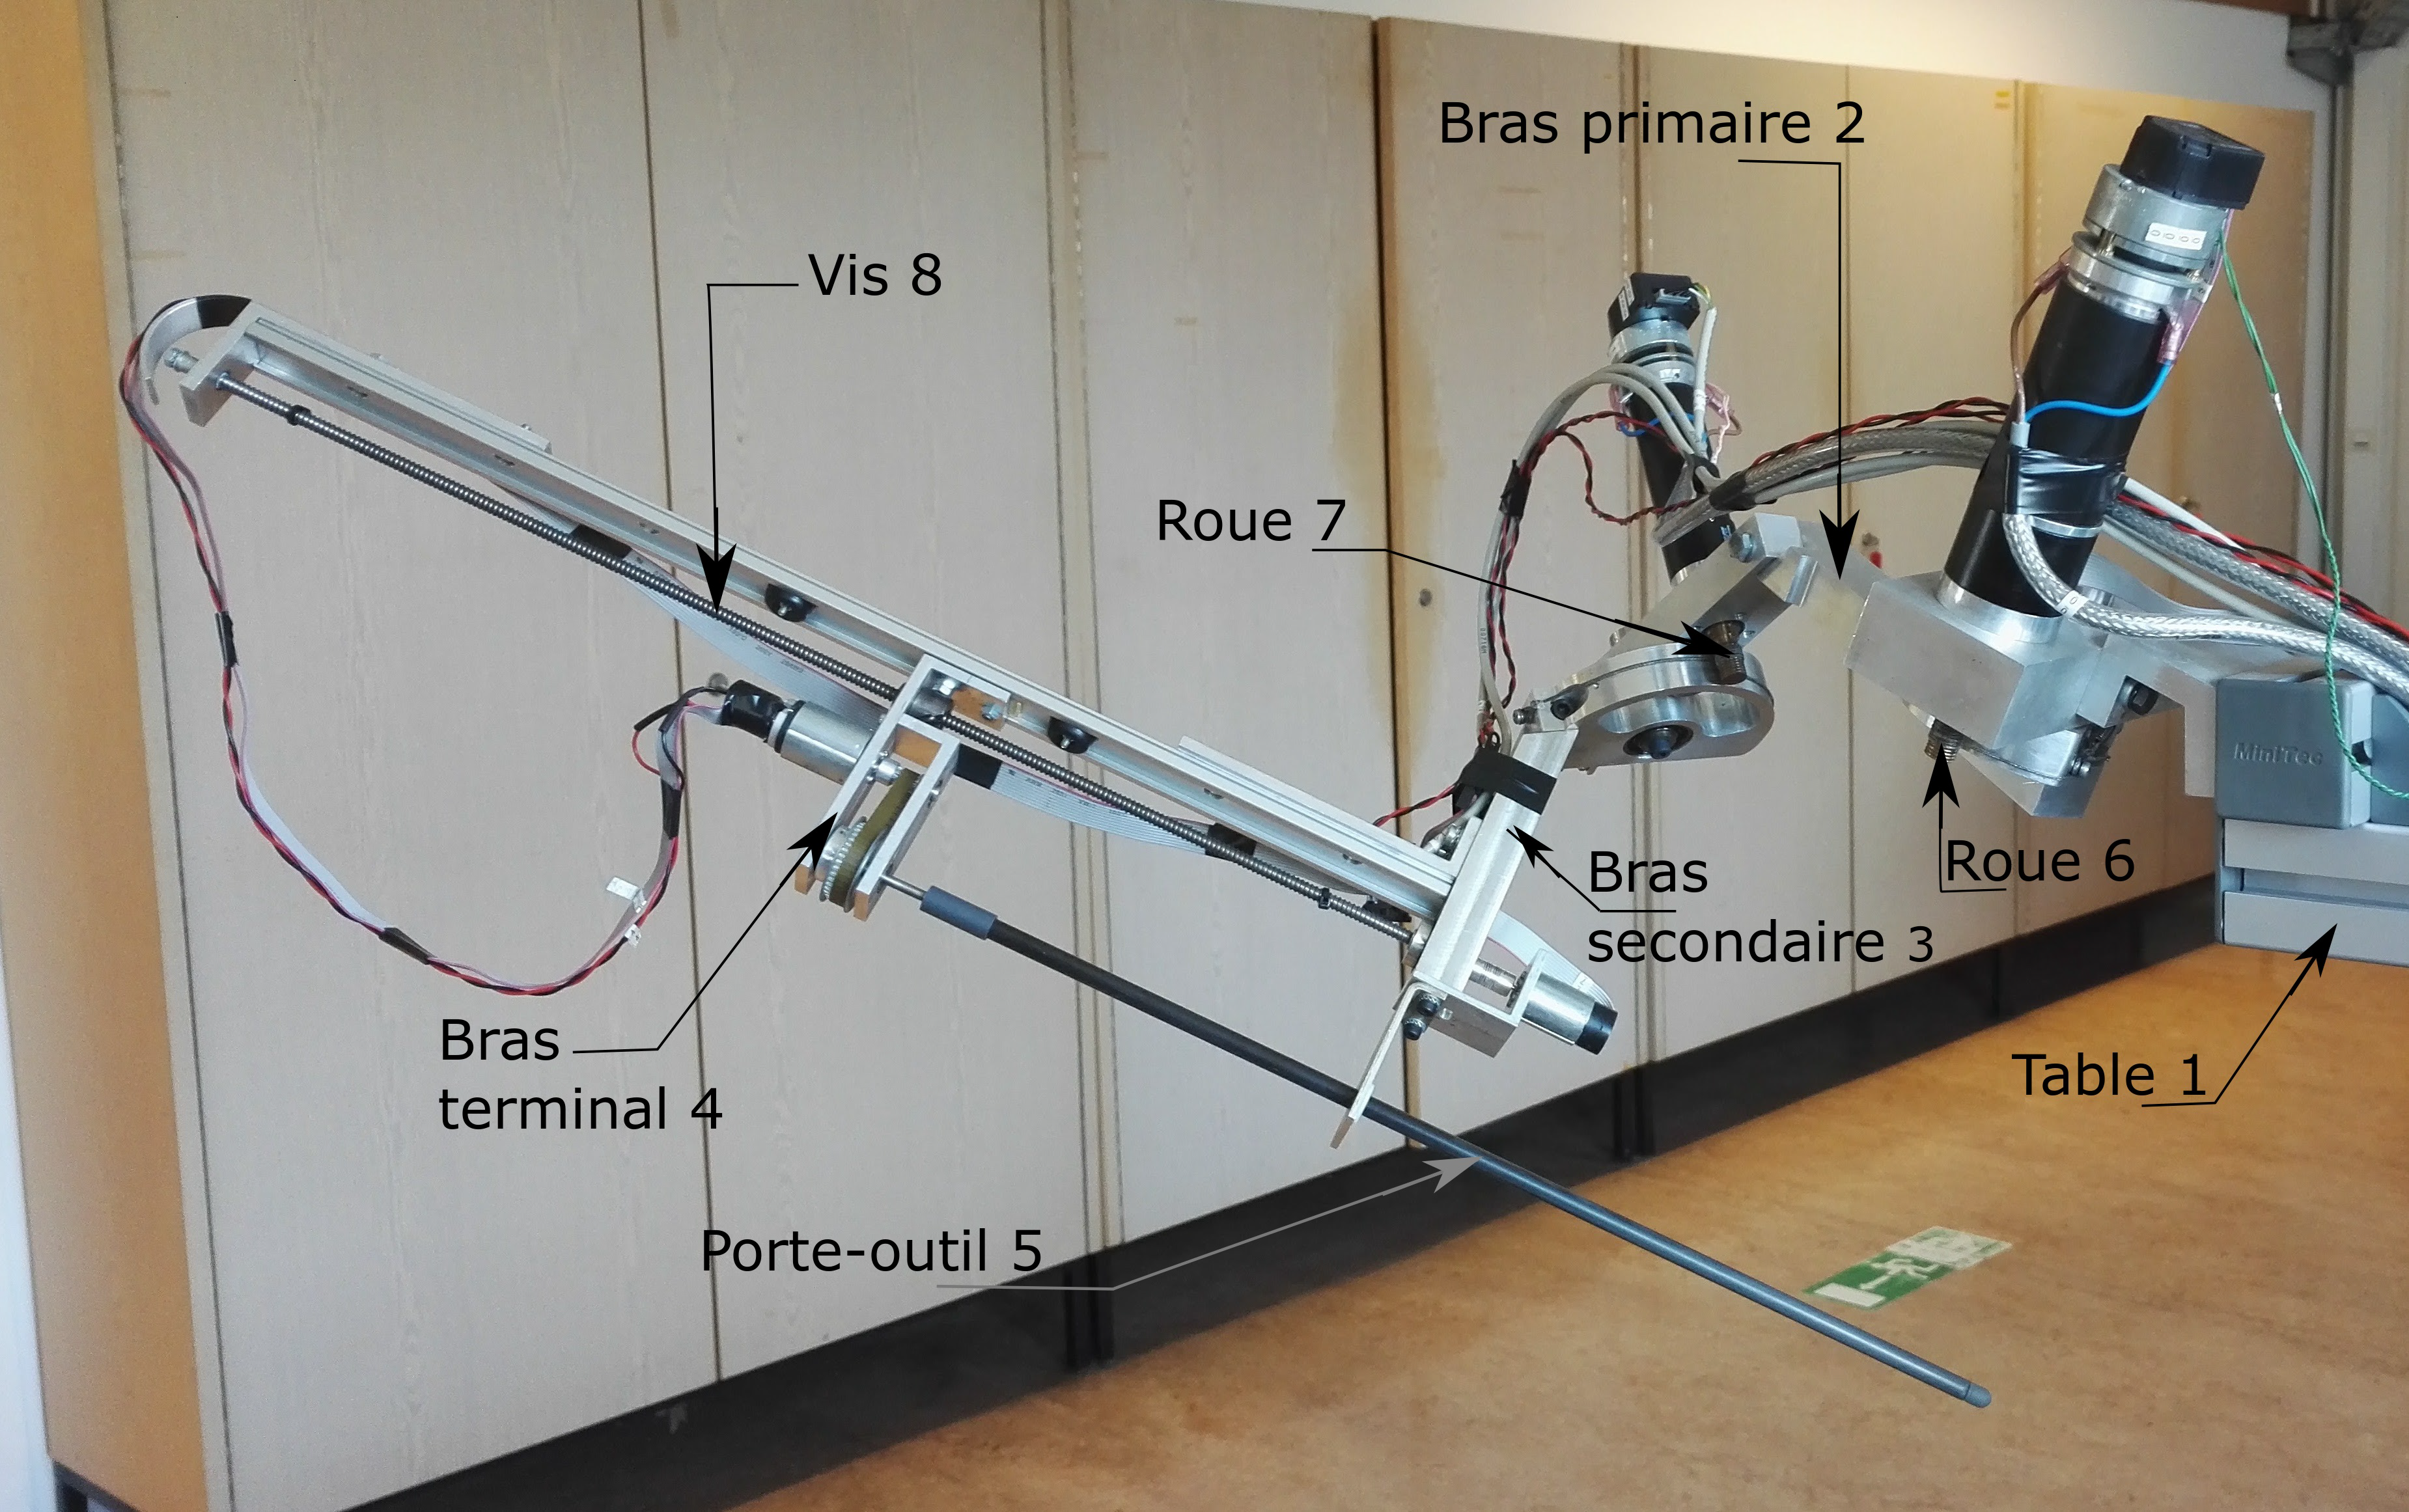
\includegraphics[width=.55\textwidth]{images/fig_00}
}%figues de la page de garde

\def\xxpied{%
Tour en fosse utilisé pour le reprofilage des roues ferroviaires\\
Concours Centrale Supelec -- PSI 2018%
}

\setcounter{secnumdepth}{5}
%---------------------------------------------------------------------------

\usepackage{bm}
\begin{document}
%\chapterimage{png/Fond_Cin}
\input{style/new_pagegarde}
\vspace{4.5cm}
\pagestyle{fancy}
\thispagestyle{plain}


\def\columnseprulecolor{\color{ocre}}
\setlength{\columnseprule}{0.4pt} 

\section{Contexte et étude préliminaire}

\begin{obj}
Valider la pertinence de l’utilisation d’une machine spéciale appelée tour en fosse pour le reprofilage
des roues ferroviaires.
\end{obj}

\subparagraph{}

\begin{itemize}
\item Pour la méthode $a$ :
\begin{itemize}
\item aller retour exploitation -- maintenance : $2t_1 = \SI{30}{min}$;
\item séparation -- assemblage des voitures : $2t_2 = \SI{60}{min}$;
\item montage -- démontage des roues : $2t_3 = \SI{480}{min}$  (le sujet est un peu ambigu);
\item reprofilage des roues : $t_3 = \SI{600}{min}$;
\end{itemize}
\item Pour la méthode $b$ :
\begin{itemize}
\item aller retour exploitation -- maintenance : $2t_1 = \SI{30}{min}$;
\item séparation -- assemblage des voitures : $2t_2 = \SI{60}{min}$;
\item reprofilage des $6 \times 3 \times 2 = 36$ roues  : $36 t_5 = \SI{540}{min} $;
\item retournement  des 6 voitures (2 retournements) : $6\times2\times t_6 =\SI{60}{min}$.
\end{itemize}
\end{itemize}
Au final : 
\begin{itemize}
\item méthode a : $t_{i1} = 2t_1 +2t_2+2t_3+t_4 = \SI{1170}{min}$;
\item méthode b : $t_{i2} = 2t_1 +2t_2+36 t_5+12 t_6 = \SI{690}{min}$;
\end{itemize}
%\end{itemize}
% $t_{i1} =2t_1+2t_2+ 2t_3 +t_4 = $ %\SI{840}{min}$.
%\item Pour la méthode $b$, $t_{i2} =2t_1+2t_2+ \left( 6\times 3 \times 2 \right)t_5 +\left( 6 \times 2 \right)t_6 =$% \SI{545}{min}$.
%\end{itemize}

Le gain de temps $\Delta t_i = t_{i1}-t_{i2}=\SI{480}{min}$ soient \SI{8}{h}. C'est autant de temps gagner sur l'exploitation de la rame. 


\section{Analyse de l’entraînement en rotation d’une roue}
\subsection{Description fonctionnelle et structurelle du tour en fosse}
\subsection{Modélisation du dispositif de mise en rotation d’une roue}


\begin{obj}
Vérifier que la modélisation et les hypothèses retenues permettent de déterminer toutes les actions mécaniques nécessaires pour dimensionner les actionneurs des chaines d’énergie.
\end{obj}

\subparagraph{}
À partir des informations données, on peut réaliser le graphe de structure suivant. 

\begin{center}
\includegraphics[width=.7\linewidth]{images/fig_02}
%\textit{}
\end{center}
\begin{multicols}{2}
\textbf{Méthode cinématique}
\begin{itemize}
\item Nombre cyclomatique $\gamma = L-S+1 $ avec $L=5$ liaisons et $S=4$ solides, on a donc $\gamma = 5-4+1=2$ et $E_c=12$ équations cinématiques.
\item Nombre d'inconnues cinématiques : 
\begin{itemize}
\item 3 liaisons pivot : $1\times 3=3$ inconnues;
\item 2 liaisons sphère-plan : $5\times 2=10$ inconnues;
\item \textbf{au total : $I_c=13$ inconnues cinématiques}.
\end{itemize}
\item Mobilités : 
\begin{itemize}
\item mobilités utiles : $m_u=2$ : entraînement des deux moteurs;
\item mobilités internes : en considérant le glissement entre la roue et les rouleaux, la roue 3, peut tourner librement. On a donc : $m_i =1$. %Dans le cas du roulement sans glissement, $m_i=3$;
\item au final, selon les hypothèses, $m=m_i+m_u=3$.
\end{itemize}
\item On a donc $h=m-I_c+E_c =3-13+12=2$.
\end{itemize}

\vfill\null
\columnbreak

\textbf{Méthode statique}
\begin{itemize}
\item 3 solides peuvent être isolés, $E_s=3\times 6 =18$ équations statiques.
\item Nombre d'inconnues statiques : 
\begin{itemize}
\item 3 liaisons pivot : $5\times 3=15$ inconnues;
\item 2 liaisons sphère-plan : $1\times 2=2$ inconnues;
\item \textbf{au total : $I_s=17$ inconnues statiques}.
\end{itemize}
\item Mobilités : $m=m_i+m_u=3$.
\item On a donc $h=m-E_S+I_s =3-18+17=2$.
\end{itemize}
\end{multicols}




%\textbf{Sans tenir compte que les solides 1, 2 et sre sont encastrés au bâti, on est dans les conditions suivantes.}
%
%\begin{center}
%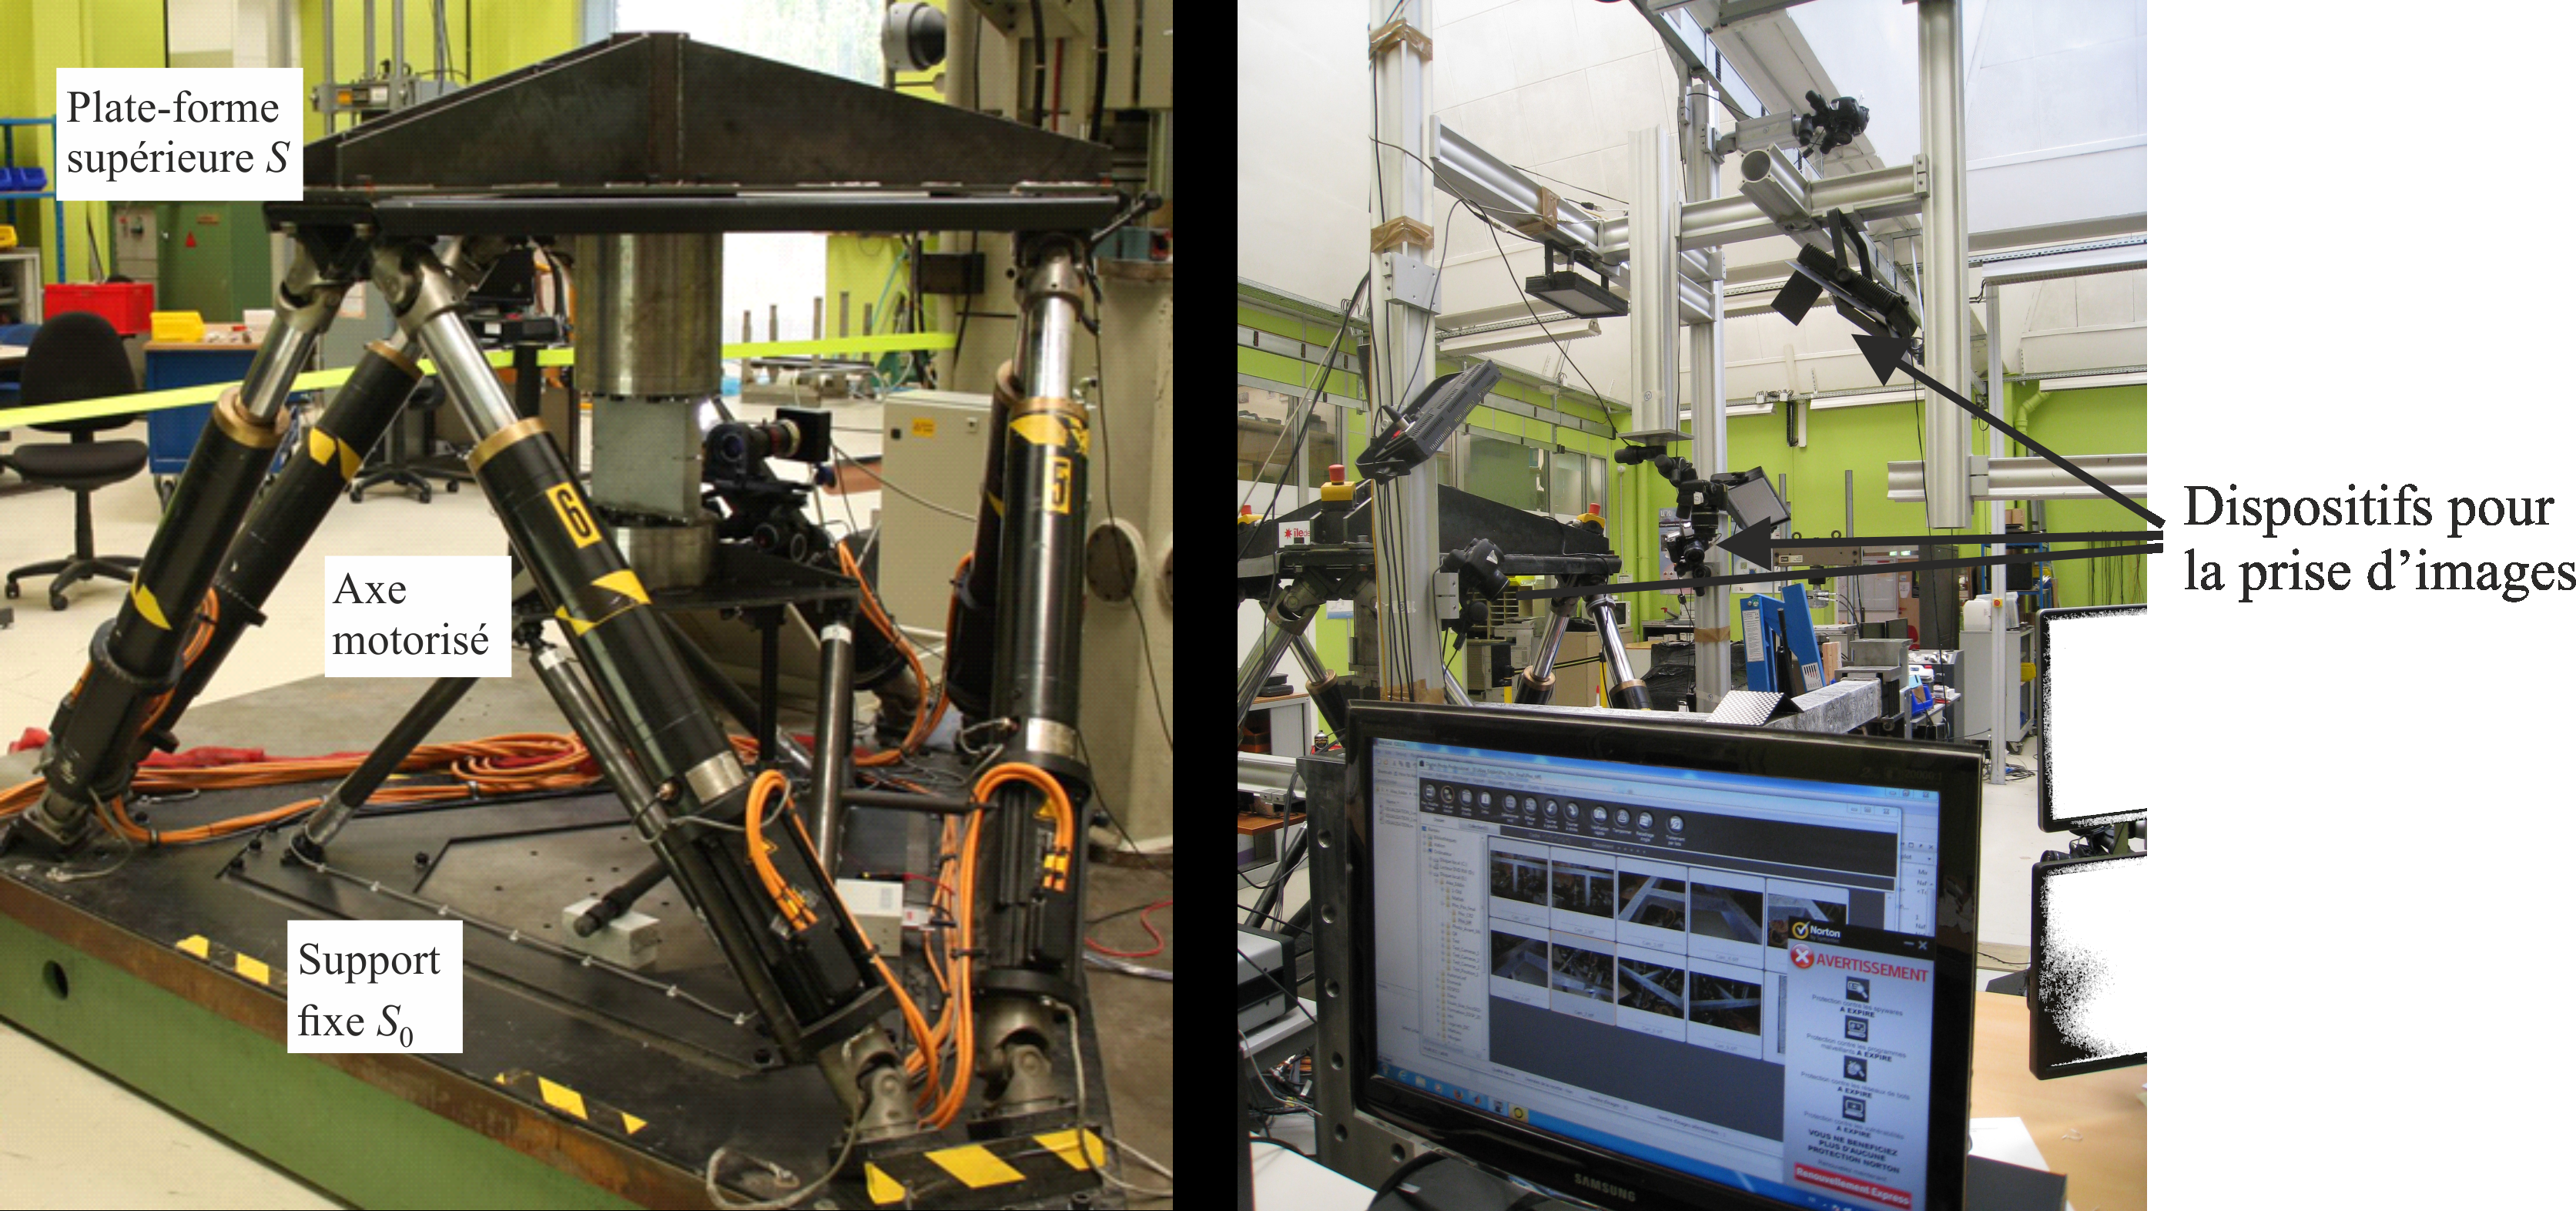
\includegraphics[width=.7\linewidth]{images/fig_01}
%%\textit{}
%\end{center}
%\begin{multicols}{2}
%\textbf{Méthode cinématique}
%\begin{itemize}
%\item Nombre cyclomatique $\gamma = L-S+1 $ avec $L=9$ liaisons et $S=7$ solides, on a donc $\gamma = 9-7+1=3$ et $E_c=18$ équations cinématiques.
%\item Nombre d'inconnues cinématiques : 
%\begin{itemize}
%\item 2 liaisons sphériques : $3\times 2=6$ inconnues;
%\item 4 liaisons pivot : $1\times 4=4$ inconnues;
%\item 1 liaison pivot glissant : 2 inconnues;
%\item 2 liaisons sphère-plan : $5\times 2=10$ inconnues;
%\item \textbf{au total : $I_c=22$ inconnues cinématiques}.
%\end{itemize}
%\item Mobilités : 
%\begin{itemize}
%\item mobilités utiles : $m_u=3$ : entrainement des deux moteurs ainsi que le déploiement du vérin;
%\item mobiltés internes : en considérant le glissement entre la roue et les rouleaux, la roue 3, ainsi que $re_1$ et $re_2$ les rouleaux peuvent tourner librement, rotation propre de la pièce 1 et de la pièce 2 autour du vecteur $\vect{AB}$. On a donc : $m_i =5$. %Dans le cas du roulement sans glissement, $m_i=3$;
%\item au final, selon les hypothèses, $m=m_i+m_u=8$.
%\end{itemize}
%\item On a donc $h=m-I_c+E_c =8-22+18=4$.
%\end{itemize}
%
%\vfill\null
%\columnbreak
%
%\textbf{Méthode statique}
%\begin{itemize}
%\item 6 solides peuvent être isolés, $E_s=6\times 6 =36$ équations statiques.
%\item Nombre d'inconnues statiques : 
%\begin{itemize}
%\item 2 liaisons sphériques : $3\times 2=6$ inconnues;
%\item 4 liaisons pivot : $5\times 4=20$ inconnues;
%\item 1 liaison pivot glissant : 4 inconnues;
%\item 2 liaisons sphère-plan : $1\times 2=2$ inconnues;
%\item \textbf{au total : $I_s=32$ inconnues statiques}.
%\end{itemize}
%\item Mobilités : $m=m_i+m_u=9$.
%\item On a donc $h=m-E_S+I_s =8-36+32=4$.
%\end{itemize}
%\end{multicols}
%
%En utilisant la condition de roulement sans glissement et la méthode cinématique, on ajoute 2 équations cinématiques et $h=3$.

\subparagraph{}
%\begin{multicols}{2}
Condition de roulement sans glissement en $I_1$ : $\vectv{I_1}{3}{re_1} = \vect{0} \Leftrightarrow \vectv{I_1}{3}{0}-\vectv{I_1}{re_1}{0} = \vect{0}$. Par suite, 
\begin{itemize}
\item $\vectv{I_1}{3}{0}=\vectv{O_3}{3}{0}+\vect{I_1 O_3}\wedge \vecto{3}{0} = R\vect{z_1} \wedge \omega_3\vect{y_0}=-R\omega_3 \vect{x_1}$;
\item $\vectv{I_1}{re_1}{0}=\vectv{O_1}{3}{0}+\vect{I_1 O_1}\wedge \vecto{3}{0} = -R_{re}\vect{z_1} \wedge \omega_{re_1}\vect{y_0}=R_{re}\omega_{re_1} \vect{x_1}$.
\end{itemize}
On a donc $-R\omega_3 -R_{re}\omega_{re_1} =0 \Leftrightarrow\dfrac{\omega_3}{\omega_{re_1}}=-\dfrac{R_{re}}{R} $.
%\end{multicols}

De même en exploitant le roulement sans glissement en $I_2$, $\dfrac{\omega_3}{\omega_{re_2}}=-\dfrac{R_{re}}{R} $. 

La condition de roulement sans glissement ajoute deux équations cinématiques. Cela supprime la mobilité de la roue 3 et impose $\omega_{re_1}=\omega_{re_2}$. 
On peut donc dire que $m'=1$ et $E_c=14$; donc $h'=1-13+14=2$. 

\subparagraph{}
Dans ces conditions précédentes, on ne peut donc pas calculer $\mathcal{C}_{m1}$ et $\mathcal{C}_{m2}$. Il faudrait donc ajouter des hypothèses complémentaires pour évaluer les couples moteurs (symétrie du problème par exemple). 

%couples $\mathcal{C}_{mi}$ ne peuvent pas être déterminés. Il faudrait imposer un taux de rotation rigoureusement identique pour $\omega_{re_1}$ et $\omega_{re_2}$. 


\subsection{Motorisation du dispositif de mise en rotation d'une roue}
\begin{obj}
Analyser la chaîne d’entraînement en rotation d’une roue et vérifier le choix de la machine électrique.
\end{obj}

\subparagraph{}
On conserve l'hypothèse que $sre$ est supposé fixe par rapport au bâti. 
On a $E_1=M_1+R_1+re_1$. Ces 3 solides sont en liaison pivot par rapport au bâti. En conséquence, 
$T\left(E_1/0\right)=T\left(M_1/0\right)+T\left(R_1/0\right)+T\left(re_1/0\right) 
= \dfrac{1}{2}J_m\omega_m^2+\dfrac{1}{2}J_{re}\omega_{re}^2+\dfrac{1}{2}J_{re}\omega_{re}^2
=\dfrac{1}{2}\left(J_m+J_{red}k^2+J_{re}k^2 \right) \omega_m^2$.

On a donc $J_{eq}=J_m+\left(J_{red}+J_{re}\right)k^2$.

\subparagraph{}
On prend le graphe de structure suivant :
\begin{center}
\includegraphics[width=.5\linewidth]{images/fig_03}
%\textit{}
\end{center}

On isole $E_1$. 

\textbf{Bilan des puissances internes :} les liaisons internes au système considérée sont considérées sans frottement. On a donc : $\mathcal{P}_{\text{int}}\left(E_1\right)=0$.

\textbf{Bilan des puissances externes :} 
\begin{itemize}
\item la puissance développée par le moteur peut s'exprimer par $\mathcal{P}\left(\text{sre}\to M_1/0\right)=C_m\omega_m$;
\item puissance développée par l'action de 3 sur $\text{re}_1$ : $\mathcal{P}\left(3\to \text{re}_1/0\right)=\torseurcin{V}{\text{re}_1}{0}\otimes\torseurstat{T}{3}{\text{re}_1}=\torseurl{k\omega_m \vect{y_0}}{kR_{re}\omega_m\vect{x_1}}{I_1}\otimes
\torseurl{-F_{z1}\vect{z_1}-F_{x1}\vect{x_1}}{\vect{0}}{I_1}= -kR_{re}F_{x1}\omega_m$.
\end{itemize}

On applique le théorème de l'énergie cinétique et $\dfrac{\dd T\left(E_1/0\right)}{\dd t}= C_m\omega_m-kR_{re}F_{x1}\omega_m \Rightarrow \dot{\omega}_m J_{eq}= C_m-kR_{re}F_{x1} \Leftrightarrow F_{x1} = \dfrac{C_m-\dot{\omega}_m J_{eq}}{kR_{re}} $.
\subparagraph{}
En isolant l'ensemble $E_2=\left\{M_2+R_2+re_2\right\}$ et en appliquant le théorème de l'énergie cinétique : $\dot{\omega}_m J_{eq}= C_m-kR_{re}F_{x2}$. Comme les caractéristiques des deux chaînes d’entraînement sont les mêmes, on a donc nécessairement $F_{x1}=F_{x2}$.

\subparagraph{}
On a vu que $\dfrac{\omega_3}{\omega_{re_1}}=-\dfrac{R_{re}}{R}$ de plus $\omega_{re_1}=k\omega_m$; donc $\omega_3= -k\dfrac{R_{re}}{R}\omega_m$. En dérivant, on a $\dot{\omega_3}= -k\dfrac{R_{re}}{R}\dot{\omega}_m$.


\subparagraph{}
\textbf{Stratégie :} on cherche à exprimer le couple moteur en fonction des grandeurs du géométriques, inertielles, ... pour cela, la roue étant en pivot d'axe $\axe{O}{y_0}$ on va réaliser un théorème du moment dynamique en $O_3$ en projection sur $\vect{y_0}$. 

On isole la roue \textbf{3}.

On réalise le bilan des actions mécaniques extérieures : 
\begin{itemize}
\item action de la pivot en $O_3$ (pas de moment en $O_3$ en projection sur $\vect{y_0}$);
\item action des liaisons sphères plans : 
\begin{itemize}
\item $\vectm{O_3}{re_1}{3}\cdot \vect{y_0} = \left(\vect{O_3 I_1} \wedge \left(  F_{x1}\vect{x_1}+F_{z1}\vect{z_1}\right) \right) \cdot \vect{y_0}
= \left(-R\vect{z_1} \wedge \left(  F_{x1}\vect{x_1}+F_{z1}\vect{z_1}\right) \right) \cdot \vect{y_0}
= -RF_{x1}$.
\item $\vectm{O_3}{re_2}{3}\cdot \vect{y_0} 
= \left(\vect{O_3 I_2} \wedge \left(  F_{x2}\vect{x_2}+F_{z2}\vect{z_2}\right) \right) \cdot \vect{y_0}
= \left(-R\vect{z_2} \wedge \left(  F_{x2}\vect{x_2}+F_{z2}\vect{z_2}\right) \right) \cdot \vect{y_0}
= -RF_{x2}$.
\end{itemize}
\item action de l'outil :
$\vectm{O_3}{\text{outil}}{3}\cdot \vect{y_0} 
= \left(\vect{O_3 C} \wedge \vectf{\text{outil}}{3} \right) \cdot \vect{y_0}
= \left(\left( -\lambda(t) \vect{y_0}-R_C(t) \vect{z_0}\right) \wedge \vectf{\text{outil}}{3} \right) \cdot \vect{y_0}
= \left( -\lambda(t) \vect{y_0}\wedge \vectf{\text{outil}}{3}-R_C(t) \vect{z_0} \wedge \vectf{\text{outil}}{3}\right)   \cdot \vect{y_0}
= \left(-R_C(t) \vect{z_0} \wedge \vectf{\text{outil}}{3} \right) \cdot \vect{y_0}
= -R_C(t)\left( \vect{y_0} \wedge \vect{z_0} \right) \cdot \vectf{\text{outil}}{3}
= -R_C(t) \vect{x_0}  \cdot \vectf{\text{outil}}{3}=R_C(t) f_{ex}
%= \left( \vectf{\text{outil}}{3} \wedge \vect{y_0}\right) \cdot \vect{O_3 C}
%= \left( \vectf{\text{outil}}{3} \wedge \vect{y_0}\right) \cdot \vect{O_3 C}
$.
\end{itemize}

Enfin, la roue étant supposée équilibrée, on a $\vectmd{O_3}{3}{0}\cdot\vect{y_0}=J_3\dot{\omega}_3$.


Le TMD appliqué en 3 en projection sur $\vect{y_0}$  est donné par 
$J_3\dot{\omega}_3=-2RF_{x1}+R_C(t) f_{ex}$. De plus, 
$\omega_3= -k\dfrac{R_{re}}{R}\omega_m$ et 
$\dot{\omega}_m J_{eq}= C_m-kR_{re}F_{x1} \Leftrightarrow F_{x1}= \dfrac{C_m-\dot{\omega}_m J_{eq}}{kR_{re}}$.

Au final :
$$-J_3k\dfrac{R_{re}}{R}\dot{\omega}_m=-2R\dfrac{C_m-\dot{\omega}_m J_{eq}}{kR_{re}}+R_C(t) f_{ex} \Leftrightarrow
C_m=\dot{\omega}_m J_{eq}
+J_3k^2\dfrac{R_{re}^2}{2R^2}\dot{\omega}_m+ \dfrac{R_C(t) kR_{re} f_{ex}}{2R}$$

et

$$C_m=\dot{\omega}_m J_{eq}
+\dfrac{kR_{re} }{2R}\left(J_3k\dfrac{R_{re}}{R}\dot{\omega}_m+ R_C(t)  f_{ex}\right).$$


%En faisant l'hypothèse que le moteur tourne dans le sens direct, la roue tourne dans le sens horaire. On peut alors déduire les signes des efforts normaux et tangentiels. Ainis, $F_{x1}=-f F_{z1}$. 
%
%
%\begin{center}
%\includegraphics[width=.5\linewidth]{images/fig_04}
%%\textit{}
%\end{center}
%
% 
%Ainsi :
%\begin{itemize}
%\item $\torseurstat{T}{re_1}{3} = \torseurl{F_{z1}\vect{z_1}+F_{x1}\vect{x_1}}{\vect{0}}{I_1}$. 
%\end{itemize}

\subparagraph{}
En utilisant l'expression précédente, le couple est maximum lorsque $R_C(t)=R_M$.

\subparagraph{}
En utilisant la décomposition du vecteur vitesse, 
$\vectv{C}{\text{outil}}{3}=\vectv{C}{\text{outil}}{0}-\vectv{C}{\text{3}}{0}$. 
D'après le document réponse, $\vectv{C}{\text{outil}}{0}=V_f(t)\vect{u}=-b\omega_3\vect{u}$. 

Par ailleurs, $\vectv{C}{\text{3}}{0}=\vectv{O}{\text{3}}{0}+\vect{CO_3}\wedge \vecto{3}{0}=\left( R_C \vect{z_0}+ \star \vect{y_0}\right)\wedge \omega_3\vect{y_0}=-R_C(t)\omega_3\vect{x_0}$.

Au final, $\vectv{C}{\text{outil}}{3}=V_f(t)\vect{u}+R_C(t)\omega_3\vect{x_0}$.

$\vectv{C}{\text{outil}}{3} \cdot \vect{x_0} = -V_C =  V_f(t)\vec t{u}\cdot \vect{x_0}+R_C(t)\omega_3 = R_C(t)\omega_3$. On a donc $V_C=-R_C(t)\omega_3$. Ainsi : 
\begin{itemize}
\item $V_C=-R_C(t)\omega_3(t)=-R_M \omega_{C_0}\Rightarrow \omega_{C_0}=-\dfrac{V_C}{R_M}$.
\item $V_C=-R_C(t)\omega_3(t)=-R_m \omega_{C_1}\Rightarrow \omega_{C_1}=-\dfrac{V_C}{R_m}$.
\end{itemize}
 
 \subparagraph{}
 
 \begin{center}
\includegraphics[width=.5\linewidth]{images/fig_05}
%\textit{}
\end{center}

Dans ces conditions, on a $\omega_3(t)=\dfrac{\omega_{C_1}-\omega_{C_0}}{t_1}t+\omega_{C_0}$.

\subparagraph{} %Q13
On a $l(t)=||\vect{C_0C}||=||\int\limits_0^t V_f(t)\vect{u} \dd t||=||\int\limits_0^t -b\omega_3(t) \vect{u} \dd t||$ 
$=||\int\limits_0^t -b\left( \dfrac{\omega_{C_1}-\omega_{C_0}}{t_1}t+\omega_{C_0}\right) \vect{u} \dd t||$

$=b|| \left(  \dfrac{\omega_{C_1}-\omega_{C_0}}{2t_1}t^2+\omega_{C_0}t\right) \vect{u} ||$.

Au final, 
$l(t)=bt \left(  \dfrac{\omega_{C_1}-\omega_{C_0}}{2t_1}t+\omega_{C_0}\right) $.


\subparagraph{} %Q14
D'après la figure, on a  $l(t_1)=||\vect{C_0C_1}||=\sqrt{\left(R_M-R_m \right)^2+e^2}$.

On a donc $l(t_1)=b \left(  \dfrac{\omega_{C_1}-\omega_{C_0}}{2t_1}t_1^2+\omega_{C_0}t_1\right) =\sqrt{\left(R_M-R_m \right)^2+e^2}$ 
$\Leftrightarrow 
  t_1 \left(\dfrac{\omega_{C_1}-\omega_{C_0}}{2}+\omega_{C_0}\right) =\dfrac{\sqrt{\left(R_M-R_m \right)^2+e^2}}{b}$.

$\Leftrightarrow 
  t_1  =\dfrac{2\sqrt{\left(R_M-R_m \right)^2+e^2}}{b\left(\omega_{C_1}+\omega_{C_0} \right)}$.


\subparagraph{} %Q15

En dérivant l'expression obtenue à la question 12, on a 
$\dot{\omega}_3(t)=\dfrac{\omega_{C_1}-\omega_{C_0}}{t_1} =  \dfrac{b\left( \omega_{C_1}+\omega_{C_0}\right)\left( \omega_{C_1}-\omega_{C_0}\right)}{2\sqrt{\left(R_M-R_m \right)^2+e^2}}  $. 

Par suite, $\dot{\omega}_3(t) =\dfrac{b\left( \omega_{C_1}^2-\omega_{C_0}^2\right)}{2\sqrt{\left(R_M-R_m \right)^2+e^2}}
=\dfrac{b\left( \dfrac{V_C^2}{R_m^2}-\dfrac{V_C^2}{R_M^2}\right)}{2\sqrt{\left(R_M-R_m \right)^2+e^2}}  $. 
Au final, 
$\dot{\omega}_3(t) 
= \dfrac{b V_C^2\left( \dfrac{1}{R_m^2}-\dfrac{1}{R_M^2}\right)}{2\sqrt{\left(R_M-R_m \right)^2+e^2}}
= \dfrac{b V_C^2\left(  R_M^2 - R_m^2 \right)}{2R_m^2R_M^2\sqrt{\left(R_M-R_m \right)^2+e^2}}
  $. 

Par ailleurs, $\dot{\omega}_m = -\dot{\omega_3} \dfrac{R}{ kR_{re}} =- \dfrac{R}{ kR_{re}}  \dfrac{b V_C^2\left(  R_M^2 - R_m^2 \right)}{2R_m^2R_M^2\sqrt{\left(R_M-R_m \right)^2+e^2}} $. 


\textit{Application numérique : } $\dot{\omega}_ m = -\SI{0.845}{rad.s^{-2}}$.

\subparagraph{} %Q16

D'après les annexes, on a $R_m=\SI{0,4}{m}$ et $V_C=\SI{400}{m.min^{-1}}$. On a donc $N_3=\dfrac{V_c}{\pi \cdot 2 R_m} = \dfrac{400}{0,8\pi} = \SI{159}{tr.min^{-1}}$. On a donc $N_m = N_3 \dfrac{R}{kR_e}=159 \dfrac{0,47}{0,1\cdot 0,175} = \SI{4275}{tr.min^{-1}}$. Le moteur doit donc pouvoir tourner au moins à cette vitesse.

Le couple moteur maximal étant de \SI{22}{Nm}, on a donc une puissane développée $P_{\text{max}}=22\times 4275 \simeq \SI{9848}{W}$.

On ne sait pas si le couple moteur maximum calculé (\SI{22}{Nm}) tient compte du rendement. 
S'il tient compte du rendement, le moteur ME\_10\_10 convient (juste). Sinon, il faudra utiliser le ME\_5\_15. 

\section{Analyse de la commande du dispositif de mise en translation de l’outil}
\begin{obj}
Analyser la chaîne d’asservissement en position et en vitesse du porte-outil afin de proposer puis de régler un correcteur permettant d’assurer le niveau de précision attendu pour le profil de la roue.
\end{obj}

\subsection{Effet de la déformation de l’outil sur la forme de la roue reprofilée}

\subparagraph{} %Q17. 

Graphiquement on a :
\begin{itemize}
\item $\Delta u_1 = \Delta z_2 \simeq \SI{5}{\mu m}$;
\item $R^2 + \Delta x_2^2 = \left(R + \Delta u_2\right)^2$ soit $\Delta u_2 = \sqrt{R^2 + \Delta x_2^2} - R = \sqrt{0,47^2 + 0,0005^2} - 0,47 \simeq \SI{0,27}{\mu m}$.%\simeq R\left(1+\dfrac{\Delta x_2^2}{2R^2}\right) - R \simeq \dfrac{\Delta x_2^2}{2R}$.
\end{itemize}
Il y a un rapport de 18,8 entre le défaut dû à la compression et celui dû à la flexion. On néglige donc ce dernier. 
 

\subsection{Analyse d’une solution avec un porte-outil fixé au bâti}
\begin{obj}
Déterminer les variations de position du point de contact $C$ entre la roue et l’outil pour une variation
sinusoïdale de l’effort perturbateur $f_c(t)$.
\end{obj}


\subparagraph{} %Q18
~\\

On isole l'outil. Celui-ci est soumis :
\begin{itemize}
\item à l'action du ressort suivant $\vect{z_0}$ : $-Kz_2(t)$;
\item à l'action de l'amortisseur $\vect{z_0}$ : $-\lambda \dot{z}_2(t)$;
\item à l'action de l'effort perturbateur $\vect{z_0}$ : $f_c(t)$. 
\end{itemize}

En appliquant le théorème de la résultante dynamique suivant $\vect{z_0}$ on obtient : $-Kz_2(t)-\lambda \dot{z}_2(t)+f_c(t)=m_2\ddot{z}_2(t)$.

En utilisant la transformée de Laplace, on obtient alors 
$-KZ_2(p)-\lambda p{Z}_2(p)+F_c(p)=m_2p^2{Z}_2(p) \Leftrightarrow S(p)=\dfrac{Z_2(p)}{F_c(p)}=\dfrac{1}{K+\lambda p  + m_2 p^2}
$.

En mettant cette fonction de transfert sous forme canonique, on a 
$K_S =1/K \simeq \SI{3,57e-8}{m.N^{-1}}$, 
$\omega_{0S}^2 = \dfrac{K}{m_2} \Rightarrow \omega_{0S}\simeq \SI{188,5}{rad.s^{-1}}$ et 
$\dfrac{2\xi_S}{\omega_{0S}} = \dfrac{\lambda}{K} \Leftrightarrow \xi_S = \dfrac{\lambda }{2\sqrt{Km_2}} \simeq 0,05$.

L'amplitude maximale est donnée par : $A_{\text{max}}=\dfrac{K_S}{2\xi_S\sqrt{1-\xi_S^2}}\simeq \dfrac{3,57\cdot 10^{-8}}{0,2\sqrt{1-0,01}}=1,8\cdot 10^{-7}$.


%%<<<<<<< HEAD
%%=======

La pulsation de résonance est donnée par $\omega_r = \omega_{0S} \sqrt{1-2\xi^2} = 188,5\sqrt{1-2\times 0,1^2}=\SI{188}{rad.s^{-1}}$.



Pour une entrée valant $f_c(t)=\left(f_{c0}+f_{c1}\sin \left(\omega t\right)\right) \mathcal{H}(t)$, en utilisant le théorème de superposition, on obtient en régime permanent le signal suivant : 
$z_2(t)=K_S f_{c0}  + f_{c1} A_{\text{max}} \sin \left(\omega_r t+\varphi\right)$ avec $\varphi=90\degres$.

Dans ces conditions on a donc $\Delta z_2 = 2 f_{c1} A_{\text{max}}\simeq \SI{3.6000e-05}{m} \simeq \SI{36}{\mu m} $. Le cahier des charges n'est donc pas respecté ($\Delta u$ doit être inférieur à $\SI{30}{\mu m}$).
\begin{center}
\includegraphics[width=.8\linewidth]{images/fig_08}
\end{center}

%%>>>>>>> a67712ce21440b340ba6bc731e97b873a885f38e

\subsection{Analyse des asservissements du porte-outil}
\subsubsection{Modélisation du mouvement pour la commande}

\begin{obj}
Modéliser le comportement dynamique de l’outil et du porte-outil, puis étudier une commande  en position $z_1(t)$ comprenant un correcteur proportionnel.
\end{obj}

\subparagraph{}

D'après le schéma-blocs $Z_1(p)=H_2(p)\left(F_m(p)+H_1(p)Z_2(p)\right)$. 
D'après la première équation différentielle, on a : $m_1p^2 Z_1(p) + \lambda pZ_1(p)+KZ_1(p)=\lambda pZ_2(p)+KZ_2(p)+F_m(p)\Leftrightarrow 
Z_1(p)\left(m_1p^2  + \lambda p+K \right)=Z_2(p)\left(\lambda p+K\right)+F_m(p)
\Leftrightarrow 
Z_1(p)= \dfrac{Z_2(p)\left(\lambda p+K\right)+F_m(p)}{m_1p^2  + \lambda p+K}$.
On a donc par identification $H_2(p)=\dfrac{1}{m_1p^2  + \lambda p+K}$ et $H_1(p)=\lambda p+K$.

D'après le schéma-blocs $Z_2(p)=H_4(p)\left(F_c(p)+H_3(p)Z_1(p)\right)$. D'après la seconde équation différentielle,  $m_2p^2 Z_2(p) + \lambda pZ_2(p)+KZ_2(p)=\lambda pZ_1(p)+KZ_1(p)+F_C(p)\Leftrightarrow Z_2(p)\left( m_2p^2  + \lambda p+K \right)=Z_1(p)\left(\lambda p+K\right)+F_C(p)\Leftrightarrow Z_2(p)=\dfrac{Z_1(p)\left(\lambda p+K\right)+F_C(p)}{ m_2p^2  + \lambda p+K}$.
On a donc par identification $H_4(p)=\dfrac{1}{m_2p^2  + \lambda p+K}$ et $H_3(p)=\lambda p+K$.

Au final, 
$$
H_1(p)=\lambda p+K \quad 
H_2(p)=\dfrac{1}{m_1p^2  + \lambda p+K} \quad 
H_3(p)=\lambda p+K  \quad 
H_4(p)=\dfrac{1}{m_2p^2  + \lambda p+K} 
$$

\subparagraph{}
En utilisant le premier modèle, on avait :
$
\left\{\begin{array}{l}
Z_1(p)=H_2(p)\left(F_m(p)+H_1(p)Z_2(p)\right) \\
Z_2(p)=H_4(p)\left(F_c(p)+H_3(p)Z_1(p)\right)
\end{array}
\right.
$. 

Ainsi, $Z_1(p)=H_2(p)\left(F_m(p)+H_1(p)\left( H_4(p)\left(F_c(p)+H_3(p)Z_1(p)\right)\right)\right) $

$=H_2(p)F_m(p)+H_1(p)H_2(p) H_4(p)F_c(p)+H_1(p)H_2(p) H_3(p)H_4(p)Z_1(p) $

$\Leftrightarrow Z_1(p)\left( 1-H_1(p)H_2(p) H_3(p)H_4(p)\right)=H_2(p)\left(F_m(p)+H_1(p)H_4(p)F_c(p)\right) $. 

En utilisant le schéma-blocs, $Z_1(p)=\left(F_c(p)N_1(p)+F_m(p)\right)N_2(p)$. 
Par identification, on obtient $N_1(p)=H_1(p)H_4(p)$ et $N_2(p)=\dfrac{H_2(p)}{1-H_1(p)H_2(p) H_3(p)H_4(p)}$.


\subparagraph{}
~\\

$N_2(p)=\dfrac{H_2(p)}{1-H_1(p)H_2(p) H_3(p)H_4(p)}$ 
$= \dfrac{\dfrac{1}{m_1p^2  + \lambda p+K}}{1-\left(\lambda p+K\right)\dfrac{1}{m_1p^2  + \lambda p+K} \left(\lambda p+K\right)\dfrac{1}{m_2p^2  + \lambda p+K}}$

$= \dfrac{1}{\left(m_1p^2  + \lambda p+K\right)- \dfrac{\left(\lambda p+K\right)^2}{m_2p^2  + \lambda p+K}}$
$= \dfrac{m_2p^2  + \lambda p+K}{\left(m_1p^2  + \lambda p+K\right)\left(m_2p^2  + \lambda p+K\right)- \left(\lambda p+K\right)^2}$

$= \dfrac{m_2p^2  + \lambda p+K}{
m_2m_1p^4  + \lambda m_1p^3+Km_1p^2+\lambda m_2p^3  + \lambda^2 p^2 +\lambda pK+Km_2p^2  + K\lambda p+K^2 - \lambda^2 p^2 -K^2 - 2\lambda p K}$

$= \dfrac{m_2p^2  + \lambda p+K}{
m_2m_1p^4  + \lambda m_1p^3+Km_1p^2+\lambda m_2p^3   +Km_2p^2 }$
$= \dfrac{m_2p^2  + \lambda p+K}{
p^2\left( m_1m_2p^2  + \left(m_1+ m_2\right) \lambda p  +K\left(m_1+m_2\right)\right) }$

$= \dfrac{m_2\left(p^2  + \dfrac{\lambda}{m_2}p+\dfrac{K}{m_2}\right)}{
p^2 m_1m_2 \left(p^2  + \dfrac{m_1+ m_2}{m_1m_2} \lambda p  +K\dfrac{m_1+m_2}{m_1m_2}\right) }$.

Par identification, on a : $A=\dfrac{1}{m_1}$, $\omega_1^2=\dfrac{K}{m_2}$, $2\xi_1\omega_1=\dfrac{\lambda}{m_2}$ et $\xi_1 = \dfrac{\lambda}{2 \omega_1 m_2}=\dfrac{\lambda}{2 \sqrt{Km_2}  } = $, $\omega_2^2=K\dfrac{m_1+m_2}{m_1m_2}$, $2\xi_2\omega_2=\lambda\dfrac{m_1+ m_2}{m_1m_2}$ et $\xi_2 = \dfrac{\lambda}{2}\sqrt{\dfrac{m_1+m_2}{m_1m_2 K}}$. 

On a donc $\xi_1=\dfrac{\lambda}{2  \sqrt{m_2K}}$ et 
$\xi_2=\lambda\dfrac{\sqrt{m_1+ m_2}}{2\sqrt{Km_1m_2}}$.



\subparagraph{}
D'après le diagramme asymptotique donné, on a nécessairement $\omega_1<\omega_2$. On peut dresser un tableau des variations à partir de la fonction de transfert $N_2(p)$. 
\begin{center}
\includegraphics[width=.7\linewidth]{images/fig_06}

\includegraphics[width=.7\linewidth]{images/fig_07}
%\textit{}
\end{center}

\subparagraph{}
Si le système n'est pas sollicité par des pulsations comprises entre 150 et \SI{250}{rad.s^{-1}}, on peut modéliser $N_2(p)$ par un double intégrateur. 
Le gain dB est donc  $20\log A - 20 \log \omega^2$.  Pour $\omega=\SI{500}{rad.s^{-1}}$ on a $20\log A - 20 \log 500^2=-182,5 \Rightarrow \log A = \dfrac{20 \log 500^2-182,5}{20}$ et $A=1,87\cdot 10^{-4}$.


\subparagraph{}

%\subparagraph{}
Dans le cas, la FTBO est de classe 2.
\begin{itemize}
\item \textbf{req 1.1} : $M\varphi = 60\degres$ : impossible à respecter la phase sera toujours de $\SI{-180}{\degres}$.
\item \textbf{req 1.2} : $\omega_{\SI{0}{dB}}=\SI{200}{rad.s^{-1}}$ : critère non respecté (cf diagramme de Bode).
\item \textbf{req 1.4} : erreur en régime permanent : $\Delta c < \SI{40}{\mu m}$ pour un échelon d'amplitude $f_{c0}=\SI{1}{kN}$ : critère non respecté (pas d'intégrateur avant la perturbation).
\item \textbf{req 1.5} : défaut de la roue $\Delta u < \SI{30}{\mu m}$ lorsque la perturbation est sinusoïdale.
\end{itemize}

La correctioin proportionnelle ne permet donc pas de respecter tous les critères du cahier des charges.

\subsubsection{Calcul des paramètres des correcteurs de la loi de commande}

\begin{obj}
Déterminer les paramètres d’une loi de commande afin de valider les performances statiques et dynamiques du cahier des charges.
\end{obj}

\subparagraph{} %
On a $\arg \left(H_{\text{BO}}(j\omega)\right)=\arg\left(AK_v \right) + \arg\left(p+\dfrac{1}{T_i}\right) + \arg\left(p+K_p\right)-3 \arg(p)$
$ =\arctan T_i\omega +\arctan\omega/K_P -270$.

On souhaite que la marge de phase soit de 60\degres soit 
$\arg \left(H_{\text{BO}}(j\omega_{\SI{0}{dB}})\right)=-120\degres$. 
On a donc 
$-120=\arctan T_i\omega_{\SI{0}{dB}} +\arctan\omega_{\SI{0}{dB}}/K_P -270 \Leftrightarrow \arctan T_i\omega_{\SI{0}{dB}} +\arctan\omega_{\SI{0}{dB}}/K_P = 150$.

Or $\tan(a+b)=\dfrac{\tan a + \tan b}{1-\tan a\tan b}$. 

On a donc $\tan 150 = \dfrac{T_i\omega_{\SI{0}{dB}} + \omega_{\SI{0}{dB}}/K_P}{1-T_i\omega_{\SI{0}{dB}}^2/K_P}$
$ \Leftrightarrow \tan 150 -\tan 150 T_i\omega_{\SI{0}{dB}}^2/K_P= T_i\omega_{\SI{0}{dB}} + \omega_{\SI{0}{dB}}/K_P $

$ \Leftrightarrow  T_i  = \dfrac{K_P\tan 150 - \omega_{\SI{0}{dB}}}{K_P\omega_{\SI{0}{dB}}+\tan 150 \omega_{\SI{0}{dB}}^2}$.


\begin{rem} D'une part, en utilisant le schéma-blocs, on a :

$H_{\text{BO}}(p)=\dfrac{K_P}{p}\dfrac{H_{\text{PI}(p)}pN_{\text{2app}}(p)}{1+H_{\text{PI}(p)}pN_{\text{2app}}(p)}$
$=\dfrac{K_P}{p}\dfrac{K_v\left(1+\dfrac{1}{Ti_ p} \right)p\dfrac{A}{p^2}}{1+K_v\left(1+\dfrac{1}{Ti_ p} \right)p\dfrac{A}{p^2}}$
$=\dfrac{K_P}{p}\dfrac{K_v\left(T_i p+1 \right){A}}{T_i p^2+K_v\left(T_i p+1 \right){A}}$.
$=\dfrac{K_P}{p}\dfrac{T_i p+1}{\dfrac{T_i}{AK_v} p^2+ T_i p+1 }$.

D'autre part, en prenant la FTBO proposée, on a : 

$H_{\text{BO}}(p)=\dfrac{AK_v\left(p+\dfrac{1}{T_i} \right)\left(p+K_p\right)}{p^3}$
$=\dfrac{AK_v}{T_i}\dfrac{T_ip^2+T_iK_pp+p+K_p }{p^3}$
$=\dfrac{AK_v}{T_iK_p}\dfrac{\dfrac{T_i}{K_p}p^2+T_ip+p+1 }{p^3}$.

La forme proposée par le sujet et la forme déterminée à parti du schéma-blocs sont donc différentes. 

\end{rem}

\subparagraph{} %Q26
%$\log\left|H_{\text{BO}}(j\omega)\right|=\log\left| AK_v \right| + \log\left|p+\dfrac{1}{T_i}\right| + \log\left|p+K_p\right|-3 \log|p|$

$H_{\text{BO}}(j\omega)=AK_v\dfrac{-\omega^2 + K_Pj\omega + \dfrac{j\omega}{T_i}+\dfrac{K_p}{T_i }}{-\omega^3}
=-\dfrac{AK_v}{\omega^3}  \left(\left(\dfrac{K_p}{T_i }-\omega^2 \right)+\left(\dfrac{1}{T_i}+ K_P\right)j\omega \right)$

On a donc 
$\log\left|H_{\text{BO}}(j\omega)\right|=\dfrac{AK_v}{\omega^3}  \sqrt{\left(\dfrac{K_p}{T_i }-\omega^2 \right)^2+\left(\dfrac{1}{T_i}+ K_P\right)^2\omega^2}$. 

Pour $\omega=\omega_{\SI{0}{dB}}$, $\log\left|H_{\text{BO}}(j\omega)\right|=1$. En conséquence, 
$\dfrac{AK_v}{\omega^3}  \sqrt{\left(\dfrac{K_p}{T_i }-\omega^2 \right)^2+\left(\dfrac{1}{T_i}+ K_P\right)^2\omega^2}=1 $

$\Leftrightarrow 
K_v  =\dfrac{\omega_{\SI{0}{dB}}^3}{A\sqrt{\left(\dfrac{K_p}{T_i }-\omega_{\SI{0}{dB}}^2 \right)^2+\left(\dfrac{1}{T_i}+ K_P\right)^2\omega_{\SI{0}{dB}}^2}}$.


\subparagraph{} %27
~\\

\noindent \hspace{.4cm} $|$ Pour $i$ allant de 0 à $N_{K_P}$ :  

\noindent \hspace{.8cm} $|$ Calcul de $K_P=i\times \Delta K_P$ 

\noindent \hspace{.8cm} $|$ Calcul de $T_i \left( K_P\right)$ 

\noindent \hspace{.8cm} $|$ Calcul de $K_v\left( K_P\right)$ 

\noindent \hspace{.8cm} $|$ Calcul de $\left| S_{K_P} \right|_{\text{max}}=\left| S\left( j \times 0\right) \right|$

\noindent \hspace{.8cm} $|$ Pour $j$ allant de 0 à $N_{\omega}$ :  

\noindent \hspace{1.2cm} $|$ Calcul de $\omega=j\times \Delta \omega$ 

\noindent \hspace{1.2cm} $|$ Calcul de $\left| S_{K_P} \right|_{\text{tmp}}=\left| S\left( j \times \omega \right) \right|$

\noindent \hspace{1.2cm} $|$ Si $\left| S_{K_P} \right|_{\text{max}}< \left| S_{K_P} \right|_{\text{tmp}}$ :

\noindent \hspace{1.6cm} $|$ $\left| S_{K_P} \right|_{\text{max}}= \left| S_{K_P} \right|_{\text{tmp}}$.

\noindent \hspace{.8cm} $|$ On stocke $\left| S_{K_P} \right|_{\text{max}}$, $K_P$, $K_v$, $T_i$ dans un liste
\subparagraph{}
~\\


\noindent \hspace{.4cm} $|$ On initialise $i_{\text{min}}$ et   $S_{\text{min}}$

\noindent \hspace{.4cm} $|$ Pour $i$ allant de 0 à $N_{K_P}$ :  

\noindent \hspace{.8cm} $|$ Si $S[i]<S_{\text{min}}$ :

\noindent \hspace{1.2cm} $|$ $i_{\text{min}}\leftarrow i$

\noindent \hspace{1.2cm} $|$ $S_{\text{min}}\leftarrow S[i]$

\noindent \hspace{.4cm} $|$ On retourne  $K_P$, $K_v$, $T_i$ associés à $i_{\text{min}}$.



\subsection{Analyse de l’influence du paramètre $b$}
\begin{obj}
Déterminer la valeur maximale de $b$ permettant de conserver la stabilité de l’asservissement.
\end{obj}



\subparagraph{}

D'après le schéma-blocs, $Q(p)=Q_c(p)-Z_2(p)H_r(p)$. 
D'après les équations données et en utilisant le théorème du retard, on a $Q(p)=Q_c(p)-Z_2(p)+Z_2(p)e^{-\tau p}=Q_c(p)-Z_2(p)\left(1-e^{-\tau p}\right)$. En conséquence, $H_r(p)=1-e^{-\tau p}$.


\subparagraph{}
$\text{FTBO}(p)=bK_f S(p)H_r(p)= \dfrac{bK_f}{K+\lambda p +m_2 p^2}\left(1-e^{-\tau p}\right) = H_2(p)\cdot H_r(p)$.

On a $G_{\text{dB}}(\omega)=G_{\text{dB2}}(\omega) + G_{\text{dBr}}(\omega)$.

$G_{\text{dBr}}(\omega) = 20\log \left|1-e^{-j\tau \omega} \right|=20\log 
\sqrt{\left( 1-\cos \left(-\tau \omega \right)\right)^2 + \left( \sin \left(-\tau \omega \right)\right)^2 } = 20\log \sqrt{2-2\cos \left( \tau \omega \right)}$.

On a donc :
\begin{itemize}
\item pour $\omega=\dfrac{k2\pi }{\tau}$ avec $k\in \mathbb{Z}^*$ et $G_{\text{dBr}}(\omega) \to -\infty $;
\item pour $\omega=\dfrac{\pi + k2\pi }{\tau}$ avec $k\in \mathbb{Z}^*$ et $G_{\text{dBr}}(\omega) = 20 \log 2$.
\end{itemize}

Le diagramme en gain montre alors l'addition d'un gain du second ordre et d'un gain périodique. Les << zéros de transmission >> correspondent aux pulsations $\omega=\dfrac{k2\pi }{\tau}$.

Pour la phase, $\varphi_{\text{BO}}\left( \omega\right)=\varphi_2\left( \omega\right)+\arg\left( 1-\cos\left( -\tau\omega\right) - j\sin\left(-\tau\omega\right)\right)$. Or $1-\cos\left( -\tau\omega\right) = 1-\cos\left( \tau \omega \right) \geq 0$. On a donc 
 $\varphi_{\text{BO}}=\varphi_2\left( \omega\right)+\arctan \left(\dfrac{\sin\left( \tau\omega\right)}{1-\cos\left( \tau\omega\right)} \right)$.

Le diagramme de  phase est la somme d'une phase d'un système du second ordre et d'un signal $\dfrac{2\pi}{\tau}$ périodique. 
\subparagraph{}
Pour garantir la stabilité en BF, il faut assurer un gain négatif en BO. D'après le diagramme de gain, le gain maximal relevé est de \SI{45}{dB}. Il faudrait donc ajouter un gain supplémentaire $b'$ tel que $20\log b' = 45$ soit $b'=10^{45/20}=177$. Au bilan, on aurait donc $b_{\text{lim}}=b' b = 177\times \dfrac{5\cdot 10^{-2}}{\pi}=
\SI{2,83}{mm.rad^{-1}}$.

Il faudrait déterminer si ine augmentation de $b$ réduit l'amortissement de l'asservissement. 
\section{Synthèse}

\subparagraph{}%32
\begin{itemize}
\item Graphiquement on mesure $\Delta z_2 = \SI{0,02}{mm}=\SI{20}{\mu m}<\SI{30}{\mu m}$. CDC OK. 
\item $\Delta e = \SI{40}{\mu m}$. CDC juste OK. 
\item La marge de phase du CDC est respectée pour $N_2(p)$ uniquement. 
\end{itemize}

Le tour permet de générer un profil de roue satisfaisant. 
\end{document}




\subparagraph{}\textit{}


\begin{center}
\includegraphics[width=\linewidth]{images/img_04}
%\textit{}
\end{center}



